% \instituicao{Federal University of Rio Grande do Norte \par 
% 			 %Exact Sciences Center\par
% 			 Department of Informatics and Applied Mathematics\par 
% 			 Computer Science Post-Graduate Program}


 
%\titulo{Uma Proposta de Metodologia para o Desenvolvimento de Aplicações
%Web Baseadas em PEWS}


   
\titulo{A Methodology for Building Service-Oriented Applications in the Presence of Non-Functional Properties} 
 
\orientador[Advisor:\vspace{1mm}]{Martin A. Musicante
(UFRN-Brazil)}
\coorientador[Co-Advisor:\vspace{1mm}]{Genoveva Vargas-Solar
(CNRS-France)}
      
\autor{Pl\'acido Ant\^onio de Souza Neto} 


\comentario{Tese submetida ao Programa de P\'os-Gradua\c c\~ao em Sistemas e
Computa\c c\~ao do Departamento de Inform\'atica e Matem\'atica Aplicada da
Universidade Federal do Rio Grande do Norte (UFRN), como requisito para a
obten\c c\~ao do grau de Doutor em Ci\^encia da Computa\c c\~ao.}

 \begin{figure}
\centering 
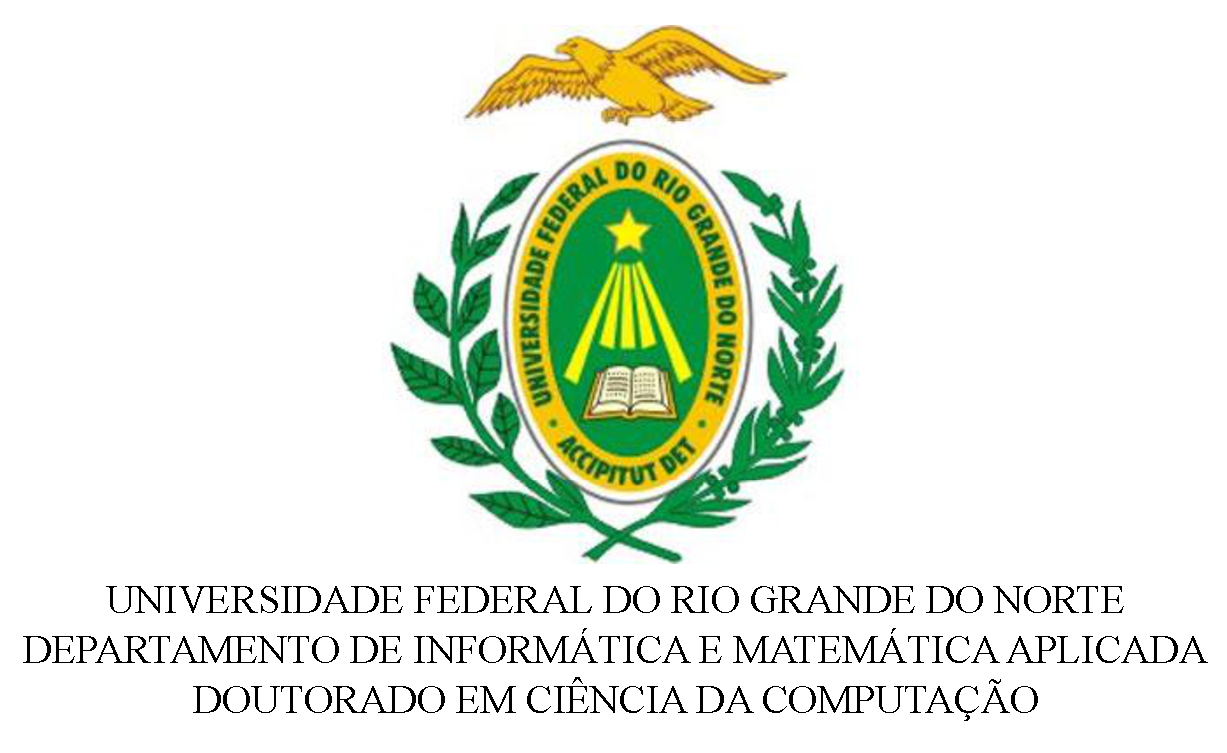
\includegraphics[width=0.75\textwidth]{chapters/figs/ufrn.pdf}
%\caption{ATL Model to Model Transformation in $\pi$SOD-M.}
%\label{fig:modelTomodelTransfomation}
\end{figure} 

% \instituicao{Federal University of Rio Grande do Norte \par 
% 			 %Exact Sciences Center\par
% 			 Computer Science and Applied Mathematics Department\par 
% 			 Systems and Computation Graduate Program \par
% 			 Doctorate in Computer Science}

%  
\local{Natal-RN / Brasil}
\data{2012} 
 
\capa   
\folhaderosto
    